\documentclass[a4paper,12pt]{scrartcl}
\usepackage{klausur}

% Parameter setzen
\setklasse{5a}
\settitel{1. Schulaufgabe im Fach Mathematik}
\setdatum{08. Dezember 2024}
\setarbeitszeit{90}

\begin{document}
\klausurtitel

\begin{aufgabe}{Berechnen Sie die Lösungen der folgenden Gleichungen.}
  \teilaufgabe[2]{Berechnen Sie $x$ für die Gleichung $x^2 - 4x + 4 = 0$.}
  \teilaufgabe[2]{Berechnen Sie $x$ für die Gleichung $x^2 - 4x + 4 = 0$.}
  \aufgabentext{Schönes Bild: \\
  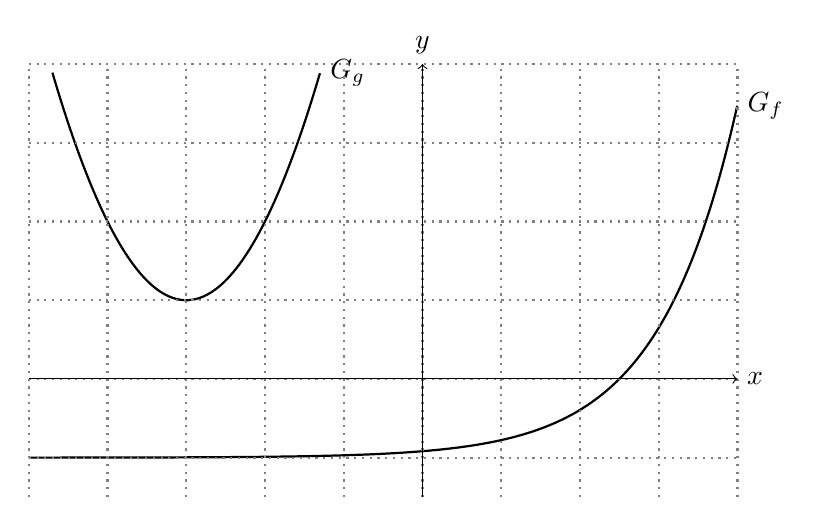
\begin{tikzpicture}[domain=-5:4]
    \draw[samples=200,smooth,domain=-4.7:-1.3,thick] plot  (\x, {(\x+3)*(\x+3)+1}) node[right] {$G_g$};
    \draw[samples=200,smooth,domain=-5:4,thick] plot  (\x, {(exp(\x-2.5)-1}) node[right] {$G_f$};
    \draw[step=1cm,gray, dotted, thick] (-5,-1.5) grid (4,4);
    \draw[->] (-5,0) -- (4,0) node[right] {$x$};
    \draw[->] (0,-1.5) -- (0,4) node[above] {$y$};
  \end{tikzpicture}\\
  }
  \teilaufgabe[3]{Was zeigt das Bild?}
\end{aufgabe}

\begin{aufgabe}{Berechne:}
  \teilaufgabe[2] {$1+2$}
  \teilaufgabe[9] { $\int_0^1 x dx$
  } 
\end{aufgabe}
\begin{aufgabe}[5]{Eine Aufgabe ohne Teilaufgaben}
  \aufgabentext{Hier steht Ihr Text.}
\end{aufgabe}

\gesamtpunkte
\end{document}
